% Options for packages loaded elsewhere
\PassOptionsToPackage{unicode}{hyperref}
\PassOptionsToPackage{hyphens}{url}
\PassOptionsToPackage{dvipsnames,svgnames,x11names}{xcolor}
%
\documentclass[
  letterpaper,
  DIV=11,
  numbers=noendperiod]{scrreprt}

\usepackage{amsmath,amssymb}
\usepackage{iftex}
\ifPDFTeX
  \usepackage[T1]{fontenc}
  \usepackage[utf8]{inputenc}
  \usepackage{textcomp} % provide euro and other symbols
\else % if luatex or xetex
  \usepackage{unicode-math}
  \defaultfontfeatures{Scale=MatchLowercase}
  \defaultfontfeatures[\rmfamily]{Ligatures=TeX,Scale=1}
\fi
\usepackage{lmodern}
\ifPDFTeX\else  
    % xetex/luatex font selection
\fi
% Use upquote if available, for straight quotes in verbatim environments
\IfFileExists{upquote.sty}{\usepackage{upquote}}{}
\IfFileExists{microtype.sty}{% use microtype if available
  \usepackage[]{microtype}
  \UseMicrotypeSet[protrusion]{basicmath} % disable protrusion for tt fonts
}{}
\makeatletter
\@ifundefined{KOMAClassName}{% if non-KOMA class
  \IfFileExists{parskip.sty}{%
    \usepackage{parskip}
  }{% else
    \setlength{\parindent}{0pt}
    \setlength{\parskip}{6pt plus 2pt minus 1pt}}
}{% if KOMA class
  \KOMAoptions{parskip=half}}
\makeatother
\usepackage{xcolor}
\setlength{\emergencystretch}{3em} % prevent overfull lines
\setcounter{secnumdepth}{5}
% Make \paragraph and \subparagraph free-standing
\ifx\paragraph\undefined\else
  \let\oldparagraph\paragraph
  \renewcommand{\paragraph}[1]{\oldparagraph{#1}\mbox{}}
\fi
\ifx\subparagraph\undefined\else
  \let\oldsubparagraph\subparagraph
  \renewcommand{\subparagraph}[1]{\oldsubparagraph{#1}\mbox{}}
\fi


\providecommand{\tightlist}{%
  \setlength{\itemsep}{0pt}\setlength{\parskip}{0pt}}\usepackage{longtable,booktabs,array}
\usepackage{calc} % for calculating minipage widths
% Correct order of tables after \paragraph or \subparagraph
\usepackage{etoolbox}
\makeatletter
\patchcmd\longtable{\par}{\if@noskipsec\mbox{}\fi\par}{}{}
\makeatother
% Allow footnotes in longtable head/foot
\IfFileExists{footnotehyper.sty}{\usepackage{footnotehyper}}{\usepackage{footnote}}
\makesavenoteenv{longtable}
\usepackage{graphicx}
\makeatletter
\def\maxwidth{\ifdim\Gin@nat@width>\linewidth\linewidth\else\Gin@nat@width\fi}
\def\maxheight{\ifdim\Gin@nat@height>\textheight\textheight\else\Gin@nat@height\fi}
\makeatother
% Scale images if necessary, so that they will not overflow the page
% margins by default, and it is still possible to overwrite the defaults
% using explicit options in \includegraphics[width, height, ...]{}
\setkeys{Gin}{width=\maxwidth,height=\maxheight,keepaspectratio}
% Set default figure placement to htbp
\makeatletter
\def\fps@figure{htbp}
\makeatother
% definitions for citeproc citations
\NewDocumentCommand\citeproctext{}{}
\NewDocumentCommand\citeproc{mm}{%
  \begingroup\def\citeproctext{#2}\cite{#1}\endgroup}
\makeatletter
 % allow citations to break across lines
 \let\@cite@ofmt\@firstofone
 % avoid brackets around text for \cite:
 \def\@biblabel#1{}
 \def\@cite#1#2{{#1\if@tempswa , #2\fi}}
\makeatother
\newlength{\cslhangindent}
\setlength{\cslhangindent}{1.5em}
\newlength{\csllabelwidth}
\setlength{\csllabelwidth}{3em}
\newenvironment{CSLReferences}[2] % #1 hanging-indent, #2 entry-spacing
 {\begin{list}{}{%
  \setlength{\itemindent}{0pt}
  \setlength{\leftmargin}{0pt}
  \setlength{\parsep}{0pt}
  % turn on hanging indent if param 1 is 1
  \ifodd #1
   \setlength{\leftmargin}{\cslhangindent}
   \setlength{\itemindent}{-1\cslhangindent}
  \fi
  % set entry spacing
  \setlength{\itemsep}{#2\baselineskip}}}
 {\end{list}}
\usepackage{calc}
\newcommand{\CSLBlock}[1]{\hfill\break\parbox[t]{\linewidth}{\strut\ignorespaces#1\strut}}
\newcommand{\CSLLeftMargin}[1]{\parbox[t]{\csllabelwidth}{\strut#1\strut}}
\newcommand{\CSLRightInline}[1]{\parbox[t]{\linewidth - \csllabelwidth}{\strut#1\strut}}
\newcommand{\CSLIndent}[1]{\hspace{\cslhangindent}#1}

\KOMAoption{captions}{tableheading}
\makeatletter
\@ifpackageloaded{bookmark}{}{\usepackage{bookmark}}
\makeatother
\makeatletter
\@ifpackageloaded{caption}{}{\usepackage{caption}}
\AtBeginDocument{%
\ifdefined\contentsname
  \renewcommand*\contentsname{Table of contents}
\else
  \newcommand\contentsname{Table of contents}
\fi
\ifdefined\listfigurename
  \renewcommand*\listfigurename{List of Figures}
\else
  \newcommand\listfigurename{List of Figures}
\fi
\ifdefined\listtablename
  \renewcommand*\listtablename{List of Tables}
\else
  \newcommand\listtablename{List of Tables}
\fi
\ifdefined\figurename
  \renewcommand*\figurename{Figure}
\else
  \newcommand\figurename{Figure}
\fi
\ifdefined\tablename
  \renewcommand*\tablename{Table}
\else
  \newcommand\tablename{Table}
\fi
}
\@ifpackageloaded{float}{}{\usepackage{float}}
\floatstyle{ruled}
\@ifundefined{c@chapter}{\newfloat{codelisting}{h}{lop}}{\newfloat{codelisting}{h}{lop}[chapter]}
\floatname{codelisting}{Listing}
\newcommand*\listoflistings{\listof{codelisting}{List of Listings}}
\makeatother
\makeatletter
\makeatother
\makeatletter
\@ifpackageloaded{caption}{}{\usepackage{caption}}
\@ifpackageloaded{subcaption}{}{\usepackage{subcaption}}
\makeatother
\ifLuaTeX
  \usepackage{selnolig}  % disable illegal ligatures
\fi
\usepackage{bookmark}

\IfFileExists{xurl.sty}{\usepackage{xurl}}{} % add URL line breaks if available
\urlstyle{same} % disable monospaced font for URLs
\hypersetup{
  pdftitle={Dynamic Group 2},
  pdfauthor={Toluwanimi Olufawo},
  colorlinks=true,
  linkcolor={blue},
  filecolor={Maroon},
  citecolor={Blue},
  urlcolor={Blue},
  pdfcreator={LaTeX via pandoc}}

\title{Dynamic Group 2}
\author{Toluwanimi Olufawo}
\date{2024-09-07}

\begin{document}
\maketitle

\renewcommand*\contentsname{Table of contents}
{
\hypersetup{linkcolor=}
\setcounter{tocdepth}{2}
\tableofcontents
}
\bookmarksetup{startatroot}

\chapter*{Preface}\label{preface}
\addcontentsline{toc}{chapter}{Preface}

\markboth{Preface}{Preface}

\section*{Intoduction}\label{intoduction}
\addcontentsline{toc}{section}{Intoduction}

\markright{Intoduction}

\textbf{Hello and Welcome!}

This blog is dedicated to showcasing the work of Group 2, a dynamic team
of dedicated students from the Visualization class at the prestigious
Oral Roberts University, Oklahoma, under the guidance of Dr.~V. Here,
you'll find weekly Quarto documents and exciting projects as they
explore the world of data visualization.

The Members of the Group 2 are

\begin{enumerate}
\def\labelenumi{\arabic{enumi}.}
\tightlist
\item
  Abigail Tako
\item
  Caleb Pena
\item
  Derrick Baruga
\item
  Toluwanimi Olufawo
\end{enumerate}

This is a Quarto book.

To learn more about Quarto books visit
\url{https://quarto.org/docs/books}.

\bookmarksetup{startatroot}

\chapter{Group 2 Blog}\label{group-2-blog}

\bookmarksetup{startatroot}

\chapter{Welcome to Group 2's Blog}\label{welcome-to-group-2s-blog}

This book is dedicated to showcasing the work of \textbf{Group 2}, a
dynamic team of dedicated students from the \textbf{Visualization} class
at the prestigious \textbf{Oral Roberts University}, Oklahoma, under the
guidance of \textbf{Dr.~V}. Here, you'll find weekly Quarto documents
and exciting projects as they explore the world of \textbf{data
visualization}.

\section{Group Members}\label{group-members}

\begin{enumerate}
\def\labelenumi{\arabic{enumi}.}
\tightlist
\item
  \textbf{Abigail Tako}
\item
  \textbf{Caleb Pena}
\item
  \textbf{Derrick Baruga}
\item
  \textbf{Toluwanimi Olufawo}
\end{enumerate}

\bookmarksetup{startatroot}

\chapter{Week2 Excel PivotTable +
Chart}\label{week2-excel-pivottable-chart}

\section{Histogram}\label{histogram}

In week 2, data sets that I am using is air quality data set. After
cleaning the data set explained below, select all the data and insert
the histogram chart to create the visualization of the data. The
variables for the histogram chart is only the ozone. From the histogram,
it shows the distribution of the ozone, most of the ozone are 1 to 25
ppm.

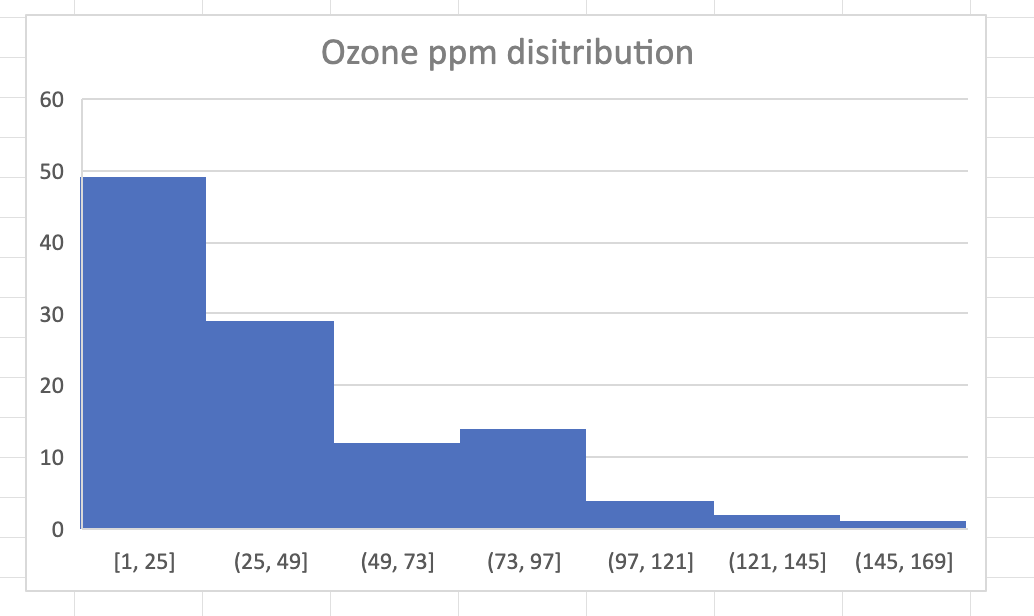
\includegraphics{Users/abigailtako/Documents/FALL 2024/Visualizations/Week 2_excelPivot_tako/histogramozone.png}

\textbf{clean data}

First, from the data, we are going to clean the data, by removing those
that are have the value NA or not available.

1. Select all the data, and search for the filter.

2. Then, it will appear the drop down menu for each column, select the
drop down menu on the first column which is Ozone

3. Select NA. To remove it, select all from the row that has NA until
the bottom and select delete rows 6-151.

4. Select the drop down menu on column Ozone, select all and apply, it
will give back the table, however there's no NA anymore on the Ozone.

Looking at the data, there still some NA on the column B for Solar.R.
Repeat the way just like before. Next, to make it earlier to read the
data, sort the day and month to be in order. Select the column for
month, click the sort from smallest to largest, do the same for day.

\section{Scatter plot}\label{scatter-plot}

Using the air quality data sets, click on column A(ozone) and D
(temperature) to show the correlation between both of them. After
clicking on both column, I'm going to insert the scatter plot. The
scatter plot shows a relationship between Ozone levels (y-axis) and
Temperature (x-axis). The general trend indicates a positive
correlation: as the temperature increases, the ozone level tends to
increase as well.

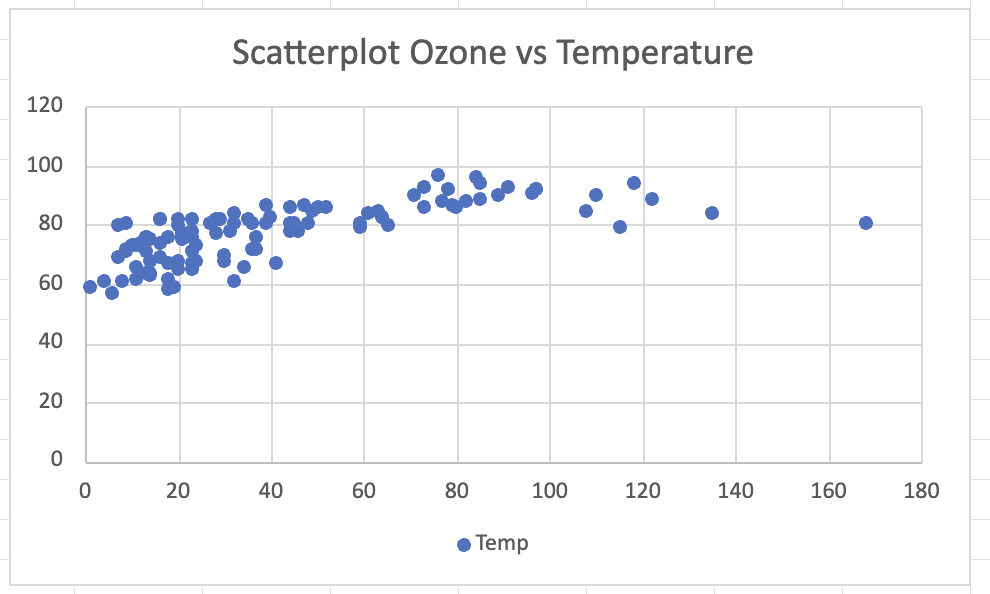
\includegraphics{Users/abigailtako/Documents/FALL 2024/Visualizations/Week 2_excelPivot_tako/scatterplotozone.png}

\section{Pivot Table \& Chart}\label{pivot-table-chart}

To make a pivot table and chart, first select all the data, and click
insert. On the let corner, it will appear the pivot menu, press that and
select the create own pivot table. I select and drag ozone, temperature,
Solar. R, and Wind to the value, for the row I'll put only the month.
Then, I change the value field settings to average, this is to provide
the average of ozone, temperature, Solar. R, and Wind monthly. After
doing the pivot table, select that pivot table and insert the pivot
chart to create the visualization.

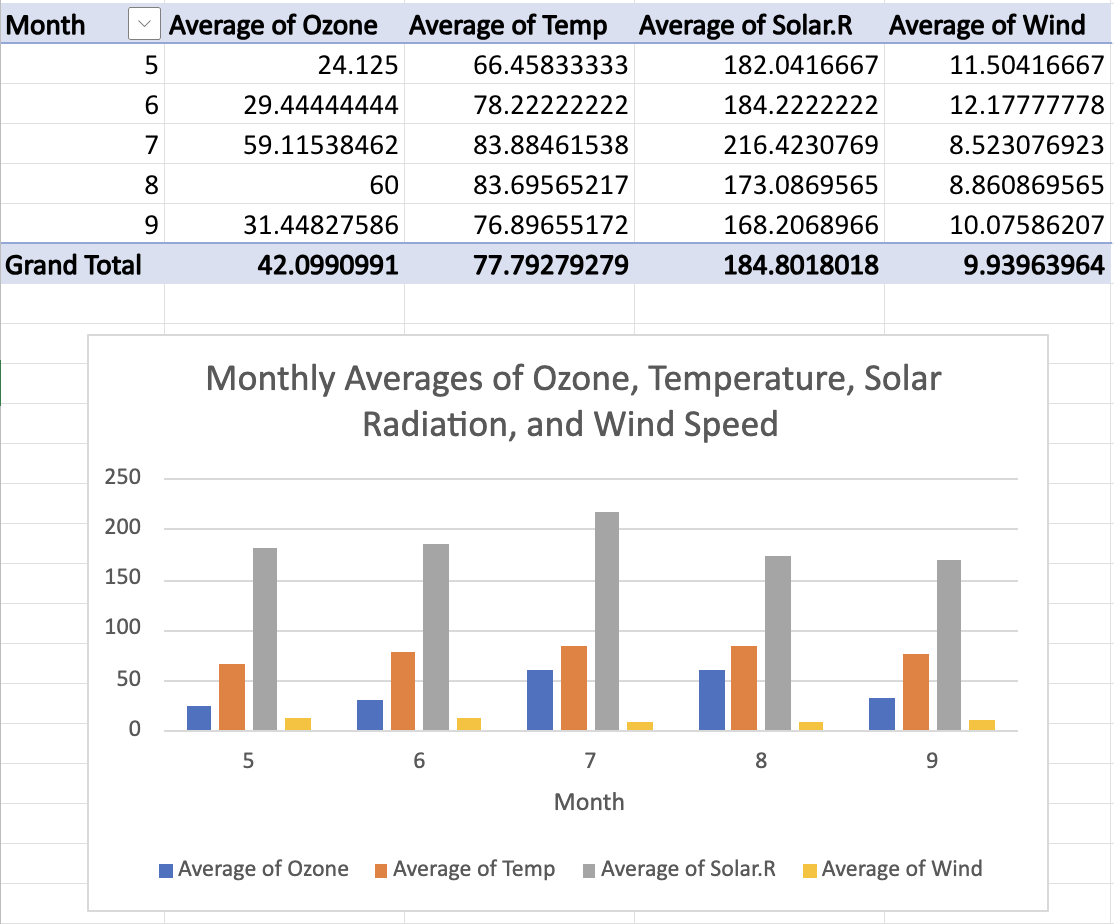
\includegraphics{Users/abigailtako/Documents/FALL 2024/Visualizations/Week 2_excelPivot_tako/pivot1.png}

From the pivot table and chart above, it shows that ozone levels appear
to increase with higher temperature and solar radiation but decrease
with higher wind speeds.

Next, I'm going to provide another pivot table, that shows the average
of ozone, temperature, Solar. R, and Wind daily from day 1 to 31. To do
that, select again the first table, the one that was cleaned, then again
select the pivot table and choose the create own pivot table.

I select and drag ozone, temperature, Solar. R, and Wind to the value,
for the row I'll put only the day. Then, I change the value field
settings to average, this is to provide the average of ozone,
temperature, Solar. R, and Wind per day.

Now, I'm going to add the pivot chart from that new pivot table. I
choose two charts, from those two I can create conclusion and better
visualizations.

From the chart presented below, the average daily of Temperature and
Wind each have a positive correlation, however not with the average
daily of Solar. R and the Ozone. Also, on day 15 it shows the lowest
average of ozone and solar. r.

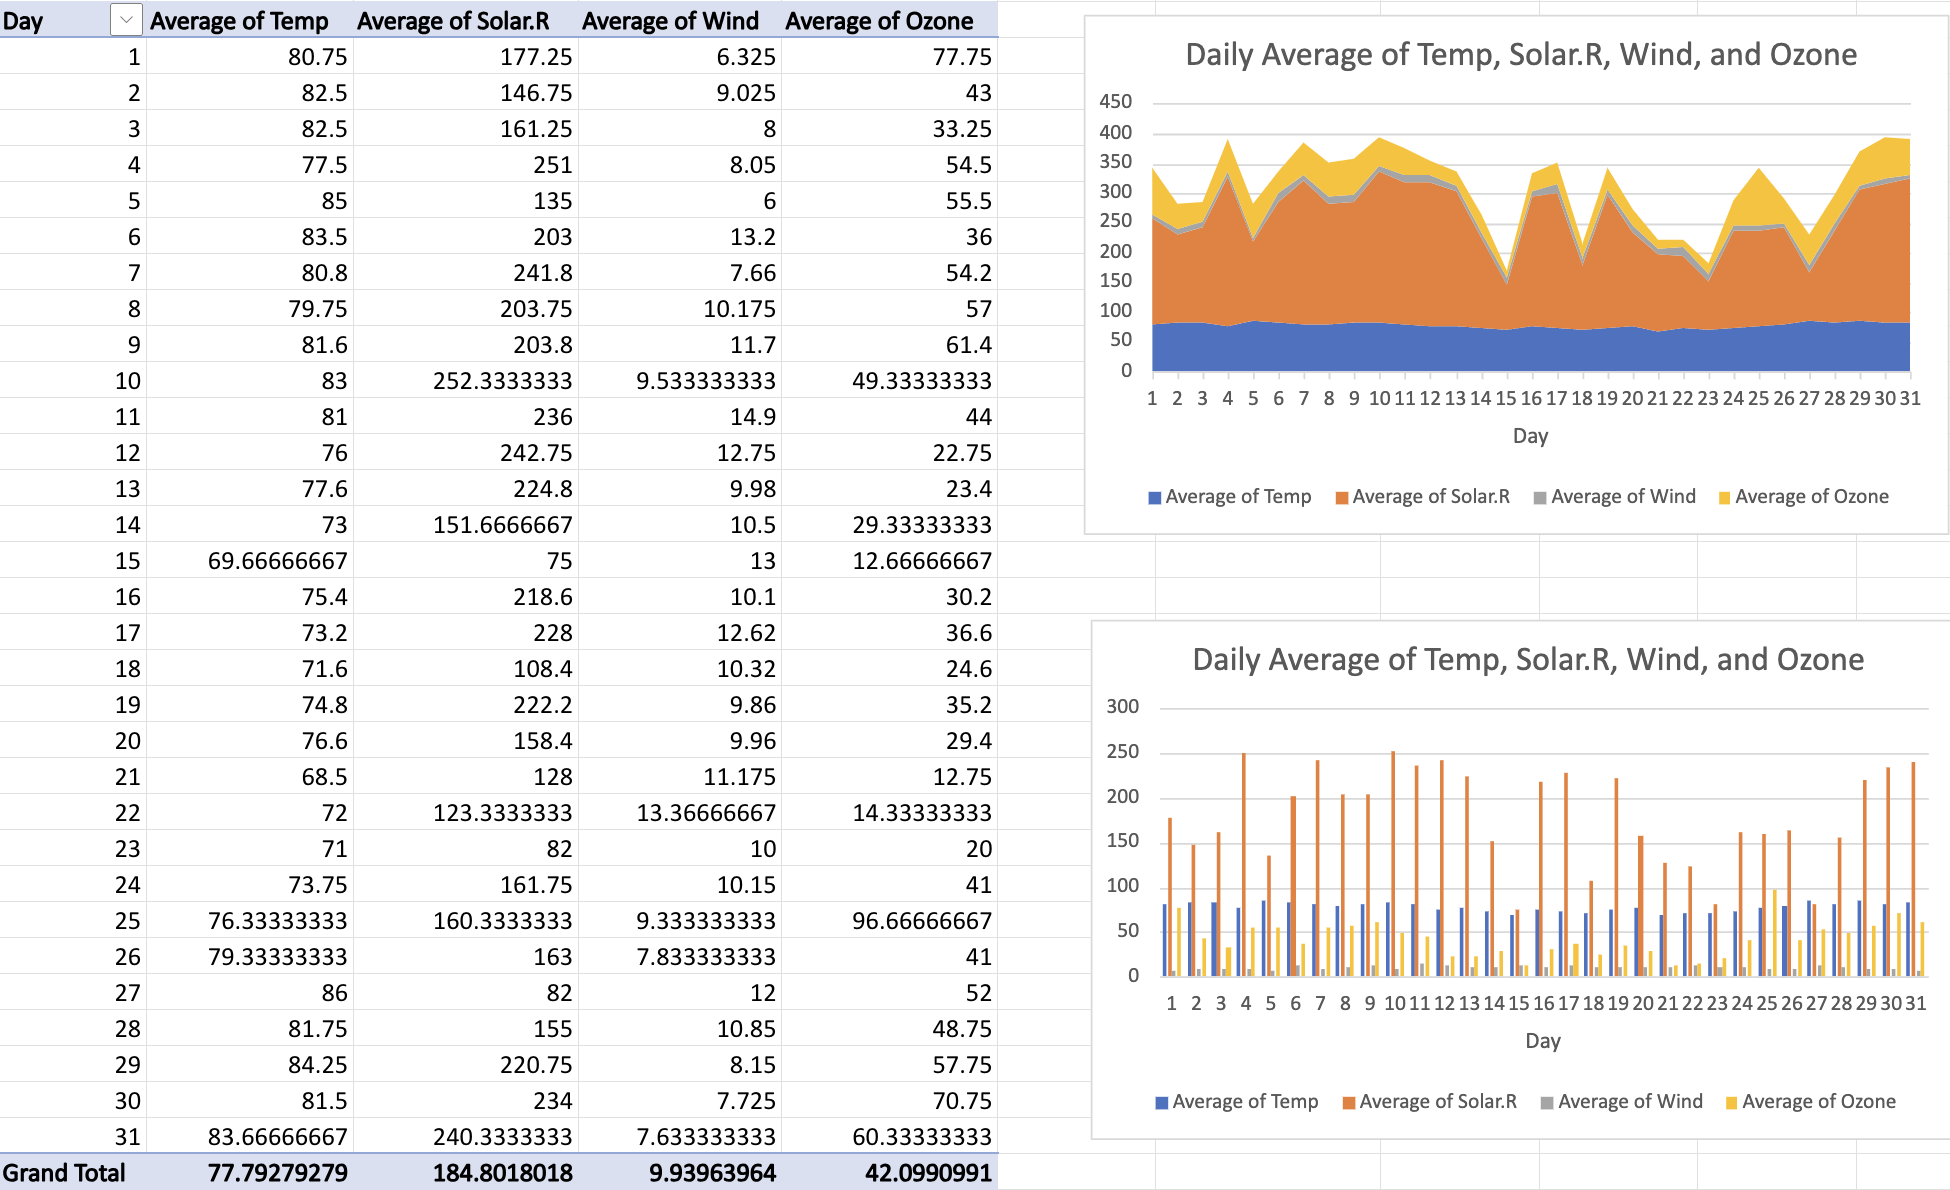
\includegraphics{Users/abigailtako/Documents/FALL 2024/Visualizations/Week 2_excelPivot_tako/pivot2.png}

Third, I'm going to make another pivot table that can show more detailed
on each month per day.I'm going to choose to present the 5th month, so
I'm going to press the drop down menu from the column ``month'' and
select only the 5. Next, the table will only provide the information
from month 5, day 1-31 and the sum of ozone, wind, temp, and solar.r.

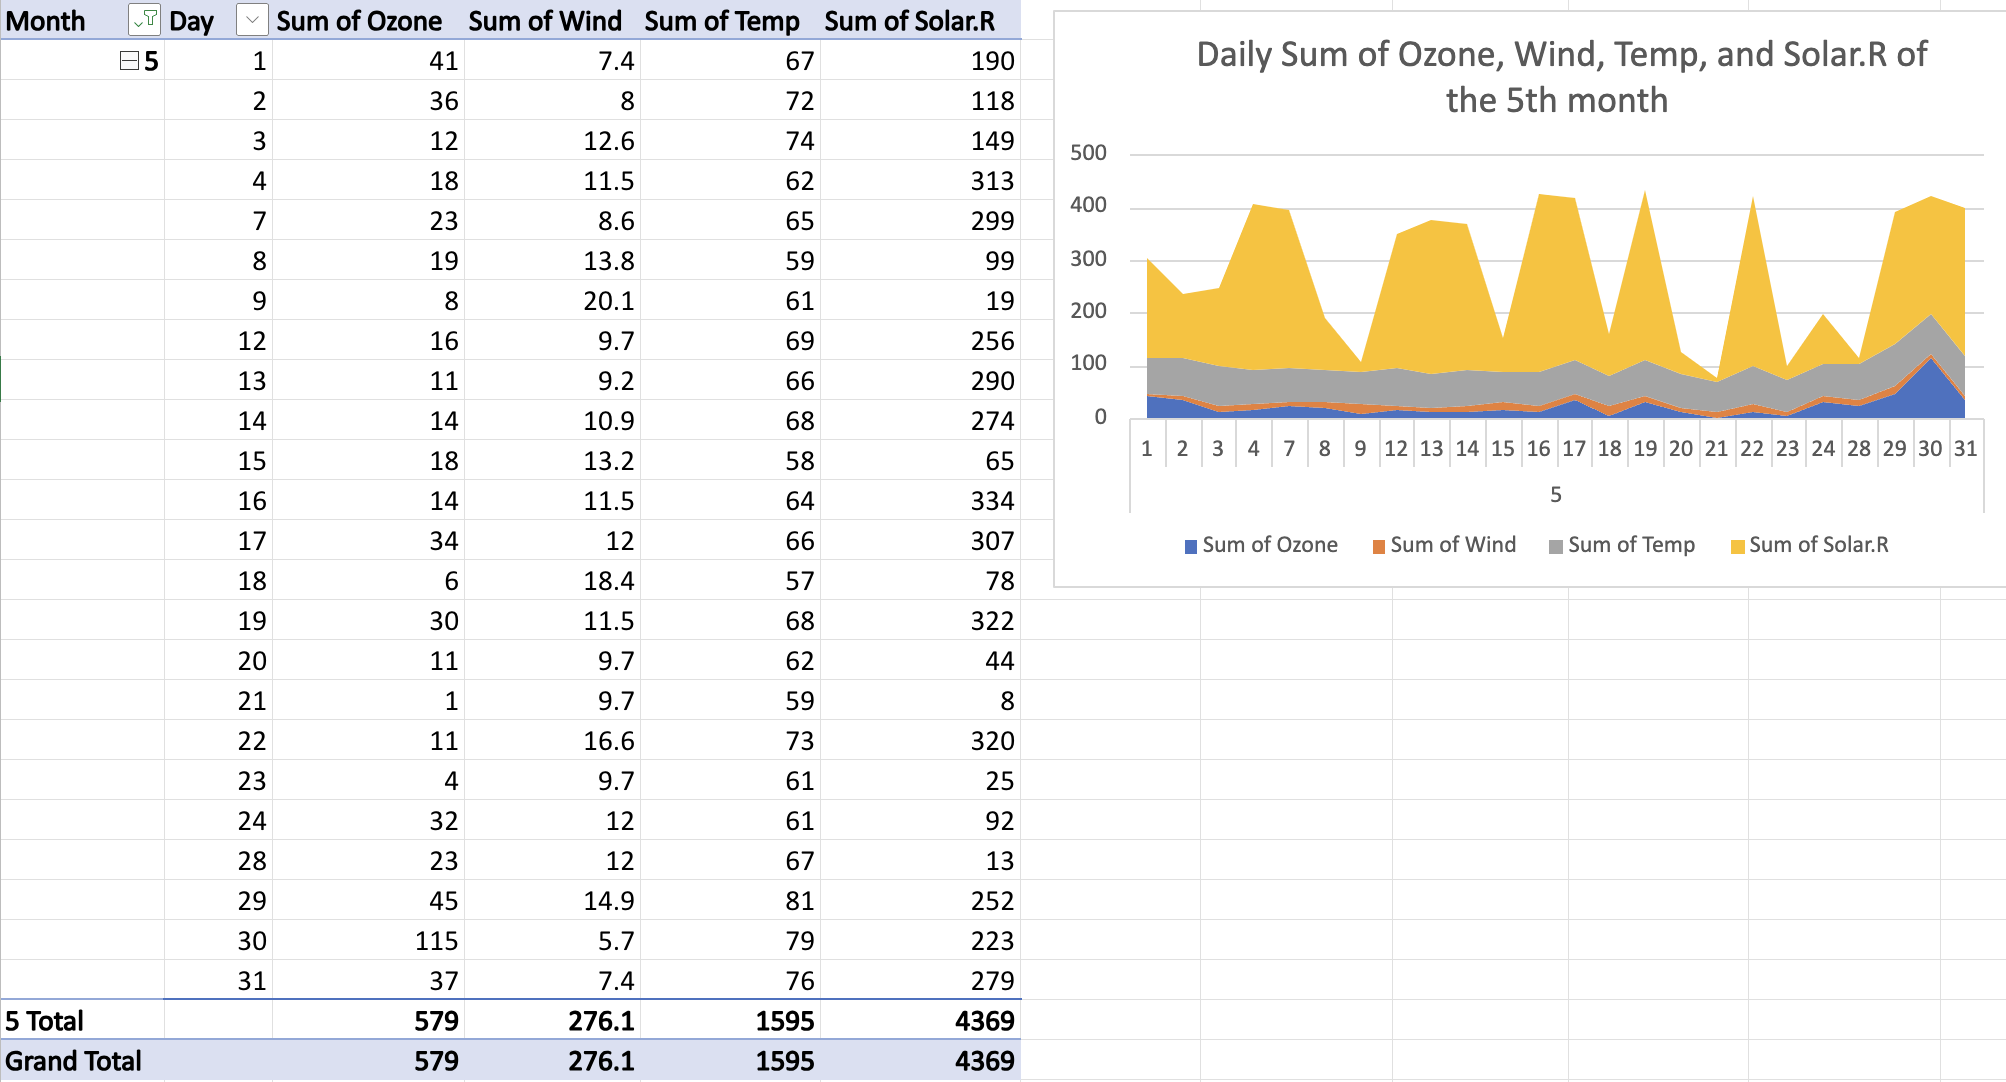
\includegraphics{Users/abigailtako/Documents/FALL 2024/Visualizations/Week 2_excelPivot_tako/pivot3.png}

From the chart, we can see that, on day 30 from the 5th month, it shows
the highest sum of ozone.

\section{Individual Project}\label{individual-project}

First, the source that I chose is National Transportation Library (NTL)
Data. There are lots of data sets from NTL, which can be access through
\url{https://ntl.bts.gov/ntl}. Then, I chose the Highway safety and
click on the motor vehicle safety data.

I'm interested in this one, because it is critical to understand trends
in road safety, which is a major public concern. The data that I collect
is from this link
\url{https://www.bts.gov/content/motor-vehicle-safety-data}. Those data
was calculated by U.S. Department of Transportation, Bureau of
Transportation Statistics.
\url{https://www.bts.gov/topics/national-transportation-statistics}

I need to rearrange the table to make it more clear, so I transpose the
from row to column.

The variables that I'm using are the year, injured, crashes, and also
vehicle. Those are the key variables that can be useful for my analysis
and visualizations.

1. Select the row and copy, then click transpose from row to column.

2. Next, select the table that has been transpose to insert the
histogram and scatter plot.

\includegraphics{Users/abigailtako/Documents/FALL 2024/Visualizations/Week 2_excelPivot_tako/histo&scatterproject.png}

From the histogram, we can look at the vehicle distribution.

From the scatter plot, we can see the correlation of each crashes,
injured, and vehicle yearly, and those three are very similar, so it
shows that each have weak correlation coefficient values, which means
that there is little to no linear relationship between those variable.

Next is to make the pivot table, insert the pivot table and I'm going to
make the year and the percentage of fatalities. Then, insert the pivot
chart.

\includegraphics{Users/abigailtako/Documents/FALL 2024/Visualizations/Week 2_excelPivot_tako/pivot1project.png}

From the pivot chart, it shows that there is a minimum fatalities
percentage on the year 2011. The percentage of fatalities in that year
reached its lowest point compared to other years in the data set. This
suggests that fewer fatalities, as a proportion of the total relevant
incidents or events, occurred in 2011 than in other years.

I add another pivot table regarding the crashes versus the percentage of
fatalities.

\includegraphics{Users/abigailtako/Documents/FALL 2024/Visualizations/Week 2_excelPivot_tako/pivot2project.png}

At first, my hypothesis was the higher number of crashes, the higher the
percentage of fatalities would be. However, looking at the chart it is
not true.

The lowest percentage of fatalities was when there were 5,377,289
crashes. The highest percentage of fatalities was when there were
6,159,350.

\section{Conclusion from Individual
Project}\label{conclusion-from-individual-project}

I take data from National Transportation Library (NTL) data that was
accessed through \url{https://ntl.bts.gov/ntl}. For my analysis, I
focused on key variables like the number of accidents, percentage of
fatalities, and safety interventions over the years. One of the
significant findings was the noticeable decrease in the percentage of
fatalities, with a minimum observed in 2011. This suggests that factors
such as improved vehicle safety features, stricter traffic laws, and
public awareness campaigns during that period may have contributed to
reducing fatalities.

Overall, this project highlights the importance of continuous monitoring
and improvement of road safety measures. Analyzing such data can guide
future strategies for reducing accidents and saving lives on the road.

\bookmarksetup{startatroot}

\chapter*{References}\label{references}
\addcontentsline{toc}{chapter}{References}

\markboth{References}{References}

\phantomsection\label{refs}
\begin{CSLReferences}{0}{1}
\end{CSLReferences}



\end{document}
